\documentclass[11pt,a4paper]{article}
\usepackage[T1]{fontenc}
\usepackage{lmodern}
\usepackage{geometry}
\geometry{margin=23mm}
\usepackage{microtype}
\usepackage{amsmath,amssymb}
\usepackage{booktabs,longtable,array,tabularx}
\usepackage{enumitem}
\usepackage{xcolor}
\usepackage{listings}
\usepackage{tikz}
\usetikzlibrary{arrows.meta,positioning,shapes.geometric,calc,fit}
\usepackage{hyperref}
\usepackage{fancyhdr}
\usepackage{caption}
\usepackage{float}
\usepackage{parskip}

\definecolor{codebg}{RGB}{247,248,250}
\definecolor{codeframe}{RGB}{210,214,220}
\definecolor{commentgreen}{RGB}{0,105,68}
\definecolor{keywordblue}{RGB}{25,70,155}
\definecolor{stringred}{RGB}{150,35,35}

\lstdefinestyle{cstyle}{
  language=C,
  basicstyle=\ttfamily\small,
  keywordstyle=\color{keywordblue}\bfseries,
  commentstyle=\color{commentgreen}\itshape,
  stringstyle=\color{stringred},
  backgroundcolor=\color{codebg},
  frame=single,
  rulecolor=\color{codeframe},
  numbers=left,
  numberstyle=\tiny\color{gray},
  numbersep=8pt,
  showstringspaces=false,
  tabsize=4,
  breaklines=true,
  columns=fullflexible,
  keepspaces=true,
  captionpos=b
}

\setlist[itemize]{topsep=3pt,itemsep=2pt}
\setlist[enumerate]{topsep=3pt,itemsep=3pt}
\setlength{\headheight}{14pt}
\setlength{\parindent}{0pt}
\emergencystretch=2em

\pagestyle{fancy}
\fancyhf{}
\lhead{SmartSafe Project}
\rhead{Servo Lock Module}
\cfoot{\thepage}

\hypersetup{
  colorlinks=true,
  linkcolor=blue!60!black,
  urlcolor=blue!60!black,
  pdftitle={SmartSafe Servo Lock Module},
  pdfauthor={Microprocessors End-Term Project}
}

\title{\textbf{SmartSafe Master Unit}\\[4pt]
\Large Complete Design and Code Explanation of the Servo Lock Module}
\author{Microprocessors End-Term Project}
\date{July 2026}

\begin{document}
\maketitle
\thispagestyle{empty}

\begin{abstract}
This report documents the servo-lock subsystem of the SmartSafe Master unit. The actuator is controlled from the ATmega32 \texttt{OC1A} output on \texttt{PD5} by Timer1 hardware PWM. The report explains how a hobby servo interprets pulse width, why a 50 Hz frame is used, how Fast PWM mode 14 is selected, how the Timer1 prescaler and \texttt{ICR1} value produce an exact 20 ms frame at an 8 MHz CPU clock, how \texttt{OCR1A} generates the 1.0 ms, 1.5 ms, and 2.0 ms control pulses, and how the angle-to-pulse conversion is derived. It also explains the independent Timer2 countdown that keeps the safe unlocked for approximately five seconds, the interaction with the main loop, startup and power-restoration behavior, sleep handling, Proteus settings, electrical limitations, and practical verification methods.
\end{abstract}

\tableofcontents
\newpage

\section{Role of the Servo in SmartSafe}
The servo represents the mechanical locking mechanism of the safe. The Master keeps the servo at the locked position during startup and ordinary operation. After a correct four-digit password is accepted, the Master commands the servo to the unlocked position, starts a five-second software countdown, blocks additional keypad activity during that interval, and then returns the actuator to the locked position.

The design separates two timing tasks:
\begin{enumerate}
  \item \textbf{Timer1} continuously generates the high-resolution PWM waveform required by the servo.
  \item \textbf{Timer2} maintains the application-level five-second open interval.
\end{enumerate}
Timer1 therefore determines the physical shaft position, while Timer2 determines how long the safe remains open.

\section{Hardware Connection}
The final signal connection is:
\begin{center}
\begin{tabular}{lll}
\toprule
Servo connection & Master connection & Purpose \\
\midrule
Control/PWM & PD5/OC1A & Timer1 compare output \\
Positive supply & +5 V & Servo electronics and motor supply \\
Ground & GND & Common electrical reference \\
\bottomrule
\end{tabular}
\end{center}

\begin{figure}[H]
\centering
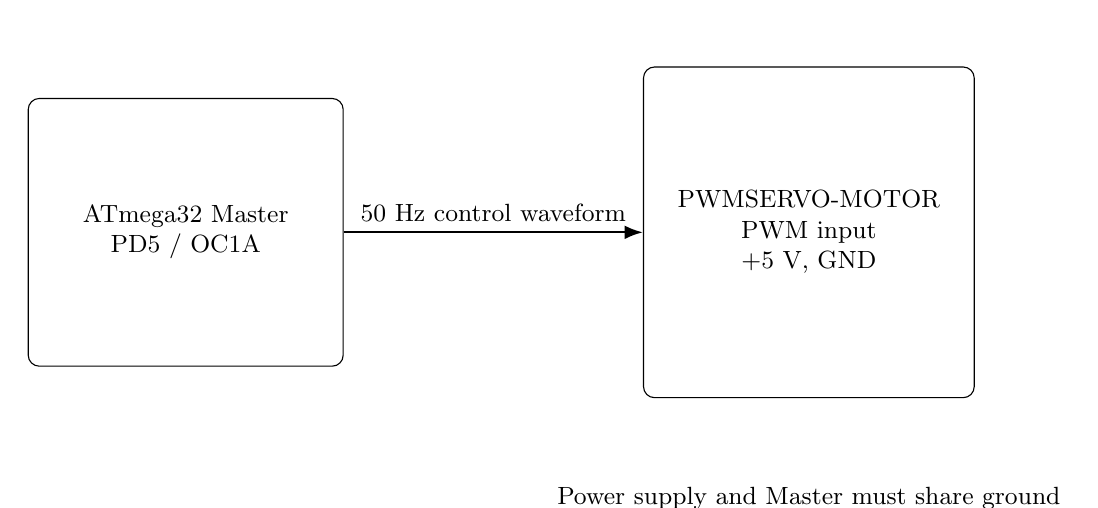
\begin{tikzpicture}[>=Latex, node distance=24mm, every node/.style={font=\small,align=center}]
\node (mcu) [draw,rounded corners,minimum width=40mm,minimum height=34mm] {ATmega32 Master\\PD5 / OC1A};
\node (servo) [draw,rounded corners,right=38mm of mcu,minimum width=42mm,minimum height=42mm] {PWMSERVO-MOTOR\\PWM input\\+5 V, GND};
\draw[->,thick] (mcu.east) -- node[above]{50 Hz control waveform} (servo.west);
\node[below=10mm of servo] {Power supply and Master must share ground};
\end{tikzpicture}
\caption{Servo control connection.}
\end{figure}

In Proteus the model can usually be powered directly from the 5 V rail. In real hardware, a servo can draw a substantial startup or stall current. It should normally use a supply sized for the motor current, a local bulk capacitor, and a 100 nF decoupling capacitor. The servo ground and microcontroller ground must remain common. The servo must not be powered from an I/O pin.

\section{How a Hobby Servo Interprets the Signal}
A standard position servo does not interpret PWM duty cycle in the same way as a DC motor controller. It primarily measures the duration of each HIGH pulse. A new pulse is sent repeatedly within a frame of approximately 20 ms:
\begin{itemize}
  \item approximately 1.0 ms HIGH: one end position, used as locked;
  \item approximately 1.5 ms HIGH: center position, used as unlocked in this project;
  \item approximately 2.0 ms HIGH: opposite end position.
\end{itemize}

\begin{figure}[H]
\centering
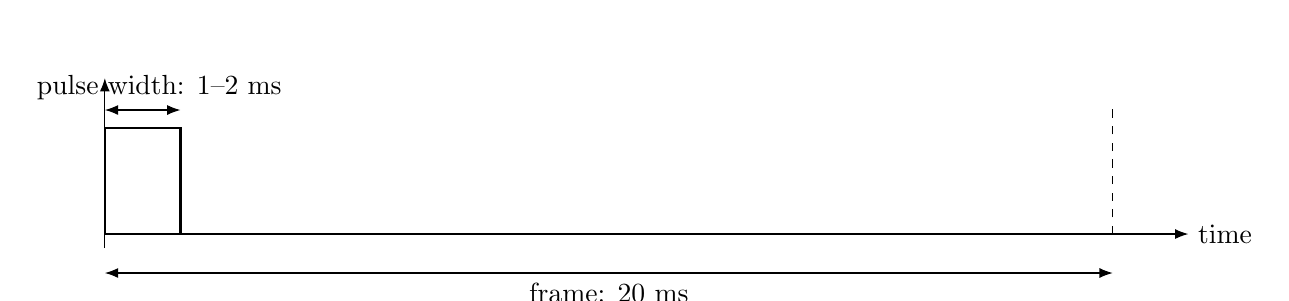
\begin{tikzpicture}[x=0.32cm,y=0.9cm,>=Latex]
\draw[->] (0,0) -- (43,0) node[right]{time};
\draw[->] (0,-0.2) -- (0,2.2);
\draw[thick] (0,0) -- (0,1.5) -- (3,1.5) -- (3,0) -- (40,0);
\draw[dashed] (40,0) -- (40,1.8);
\draw[<->] (0,1.75) -- node[above,pos=0.72]{pulse width: 1--2 ms} (3,1.75);
\draw[<->] (0,-0.55) -- node[below]{frame: 20 ms} (40,-0.55);
\end{tikzpicture}
\caption{Servo waveform concept. The illustrated pulse is schematic; the frame repeats continuously.}
\end{figure}

For the selected 20 ms frame, the nominal duty cycles are only 5 percent, 7.5 percent, and 10 percent. The pulse width, rather than the percentage itself, is the meaningful control quantity.

\section{Why Timer1 Is Used}
Timer1 is a 16-bit timer/counter. A 20 ms frame with one-microsecond resolution requires 20,000 timer counts, which is larger than the 256-count range of an 8-bit timer. Timer1 can represent this period directly and provides a dedicated hardware compare output on \texttt{OC1A/PD5}. Once configured, the waveform is generated in hardware without software toggling and without timing jitter from the main loop.

\section{Timer1 Register Configuration}
The initialization code is:
\begin{lstlisting}[style=cstyle,caption={Servo initialization and Timer1 configuration.}]
void servo_init(void)
{
    SERVO_DDR |= (1U << SERVO_PIN);

    TCCR1A = (1U << COM1A1) | (1U << WGM11);
    TCCR1B = (1U << WGM13)  |
             (1U << WGM12)  |
             (1U << CS11);

    ICR1  = 19999U;
    servo_lock();
}
\end{lstlisting}

\subsection{PD5 data direction}
\begin{lstlisting}[style=cstyle]
SERVO_DDR |= (1U << SERVO_PIN);
\end{lstlisting}
sets \texttt{DDRD5=1}. This makes \texttt{PD5} an output. When the compare-output function is enabled, Timer1 controls the pin automatically.

\subsection{Waveform-generation mode}
The waveform-generation bits are distributed across two registers:
\begin{center}
\begin{tabular}{ccccc}
\toprule
Bit & WGM13 & WGM12 & WGM11 & WGM10 \\
\midrule
Selected value & 1 & 1 & 1 & 0 \\
\bottomrule
\end{tabular}
\end{center}
This binary pattern, \texttt{1110}, selects Fast PWM mode 14. In this mode:
\begin{itemize}
  \item \texttt{ICR1} defines TOP and therefore the frame period;
  \item \texttt{OCR1A} defines the compare point and therefore the HIGH-pulse width;
  \item the counter runs from 0 through \texttt{ICR1}, then restarts at 0.
\end{itemize}

The register assignments are:
\begin{lstlisting}[style=cstyle]
TCCR1A = (1U << WGM11);
TCCR1B = (1U << WGM13) | (1U << WGM12);
\end{lstlisting}
with the compare-output and prescaler bits added to the same values.

\subsection{Non-inverting OC1A output}
The compare-output bits are:
\begin{center}
\begin{tabular}{ccc}
\toprule
COM1A1 & COM1A0 & Behavior in Fast PWM \\
\midrule
1 & 0 & Clear OC1A on compare match; set OC1A at BOTTOM \\
\bottomrule
\end{tabular}
\end{center}
Therefore the output becomes HIGH when the timer starts a new frame and becomes LOW when \texttt{TCNT1=OCR1A}. The HIGH duration is approximately \texttt{OCR1A} timer ticks.

\subsection{Clock prescaler}
The clock-select field is:
\begin{center}
\begin{tabular}{cccc}
\toprule
CS12 & CS11 & CS10 & Timer1 clock \\
\midrule
0 & 1 & 0 & $F_{CPU}/8$ \\
\bottomrule
\end{tabular}
\end{center}
At \(F_{CPU}=8\,000\,000\) Hz,
\[
f_{T1}=\frac{8\,000\,000}{8}=1\,000\,000\text{ Hz}.
\]
The duration of one timer count is therefore
\[
T_{tick}=\frac{1}{1\,000\,000}=1\ \mu\text{s}.
\]
This prescaler is especially convenient because timer counts and pulse width in microseconds have the same numerical value.

\section{Calculation of ICR1 and the 50 Hz Frame}
In Fast PWM mode 14, the frame period is
\[
T_{PWM}=\frac{N(1+ICR1)}{F_{CPU}},
\]
where \(N\) is the prescaler. Solving for \texttt{ICR1} with a 20 ms target gives
\[
ICR1=\frac{T_{PWM}F_{CPU}}{N}-1
     =\frac{0.020\times8\,000\,000}{8}-1
     =19\,999.
\]
The resulting frequency is
\[
f_{PWM}=\frac{8\,000\,000}{8(19\,999+1)}=50\text{ Hz}.
\]
The code therefore uses:
\begin{lstlisting}[style=cstyle]
ICR1 = 19999U;
\end{lstlisting}

\section{Calculation of OCR1A Values}
Because one Timer1 count equals one microsecond:
\begin{center}
\begin{tabular}{cccc}
\toprule
Commanded position & Pulse width & OCR1A & Duty cycle \\
\midrule
Locked, 0 degrees & 1.0 ms & 1000 & 5.0 percent \\
Unlocked, 90 degrees & 1.5 ms & 1500 & 7.5 percent \\
Opposite end, 180 degrees & 2.0 ms & 2000 & 10.0 percent \\
\bottomrule
\end{tabular}
\end{center}

The conversion function is:
\begin{lstlisting}[style=cstyle,caption={Angle-to-pulse conversion.}]
void servo_set(uint8_t angle)
{
    if (angle > 180U)
        angle = 180U;

    OCR1A = (uint16_t)(1000UL +
            ((uint32_t)angle * 1000UL) / 180UL);
}
\end{lstlisting}

The linear mapping is
\[
OCR1A=1000+\frac{angle\times1000}{180}.
\]
Examples are:
\[
angle=0:\quad OCR1A=1000,
\]
\[
angle=90:\quad OCR1A=1000+\frac{90\times1000}{180}=1500,
\]
\[
angle=180:\quad OCR1A=2000.
\]
The multiplication is explicitly promoted to 32 bits so that the intermediate product cannot overflow an 8-bit or 16-bit object.

\section{Lock and Unlock Functions}
The public interface deliberately hides numeric angles from the application:
\begin{lstlisting}[style=cstyle]
void servo_lock(void)
{
    servo_set(0U);
}

void servo_unlock(void)
{
    servo_set(90U);
}
\end{lstlisting}
The project defines 0 degrees as locked and 90 degrees as unlocked. This convention can be reversed mechanically without changing the Timer1 calculations; only the two commanded angles would need adjustment.

\section{Five-Second Open Interval}
Timer1 controls position but does not count the five-second access interval. The main application uses:
\begin{lstlisting}[style=cstyle]
servo_unlock();
servo_open = 1U;
servo_counter = SERVO_OPEN_SEC;  /* 5 */
\end{lstlisting}
Timer2 decrements \texttt{servo\_counter} approximately once per second. The main loop then detects zero and locks the servo:
\begin{lstlisting}[style=cstyle]
if (servo_open && servo_counter == 0U) {
    servo_lock();
    servo_open = 0U;
    redraw = 1U;
}
\end{lstlisting}
Keeping the actual actuator command in the main loop prevents complex peripheral operations from being performed inside an interrupt service routine.

\section{Timer2 Calculation for the Open-Time Counter}
Timer2 is configured in CTC mode:
\begin{lstlisting}[style=cstyle]
OCR2 = 77U;
TCCR2 = (1U << WGM21) |
        (1U << CS22)  |
        (1U << CS21)  |
        (1U << CS20);
TIMSK |= (1U << OCIE2);
\end{lstlisting}
The clock-select bits \texttt{111} select a prescaler of 1024. The compare period is
\[
T_{match}=\frac{1024(77+1)}{8\,000\,000}
         =9.984\text{ ms}.
\]
Ten compare matches produce
\[
10\times9.984=99.84\text{ ms},
\]
and ten 100 ms software intervals produce
\[
10\times99.84=998.4\text{ ms}.
\]
Thus the nominal five-second interval is approximately
\[
5\times0.9984=4.992\text{ s}.
\]
The error is only about \(-0.16\) percent, which is insignificant for a safe-door demonstration.

\section{Main-Loop Sequence}
A successful password causes the following sequence:
\begin{enumerate}
  \item reset the internal EEPROM failed-attempt count;
  \item store a successful-login event in the external EEPROM;
  \item send \texttt{LOGIN\_OK} through USART to the Slave;
  \item call \texttt{servo\_unlock()}, loading \texttt{OCR1A=1500};
  \item set \texttt{servo\_open=1} and \texttt{servo\_counter=5};
  \item prevent keypad input and inactivity sleep while the door is open;
  \item decrement the counter through Timer2;
  \item call \texttt{servo\_lock()} when the counter reaches zero.
\end{enumerate}

\section{Startup, Sleep, and Power-Failure Behavior}
\subsection{Startup}
\texttt{servo\_init()} configures Timer1 and immediately calls \texttt{servo\_lock()}. The actuator therefore begins in a defined safe position rather than using an undefined compare value.

\subsection{Normal inactivity sleep}
Normal inactivity sleep is allowed only when \texttt{servo\_open=0}. The safe therefore cannot enter Power-down while the door-open countdown is active.

\subsection{Confirmed power failure}
Before power-failure standby, the firmware stops Timer1 and forces the servo signal pin low. After monitored voltage restoration, \texttt{servo\_init()} is called again, which reconstructs the 50 Hz waveform and locks the safe. This fail-safe restart behavior is intentional.

\section{Proteus Configuration and Test Procedure}
Use the following settings:
\begin{itemize}
  \item ATmega32 clock property: 8 MHz;
  \item servo signal: PD5/OC1A;
  \item frame period: 20 ms or frequency 50 Hz;
  \item minimum pulse: approximately 1 ms;
  \item center pulse: approximately 1.5 ms;
  \item maximum pulse: approximately 2 ms;
  \item initial angle: locked position.
\end{itemize}

A logic analyzer should show a 20 ms period. In the locked state the HIGH pulse should be about 1 ms. After password acceptance it should become about 1.5 ms for approximately five seconds and then return to 1 ms.

\section{Common Failure Modes}
\begin{longtable}{p{0.31\textwidth}p{0.61\textwidth}}
\toprule
Symptom & Likely cause and correction \\
\midrule
\endhead
Servo remains near 180 degrees & MCU clock does not match \texttt{F\_CPU}, Timer1 prescaler is wrong, or the Proteus pulse limits do not match 1--2 ms. \\
Movement lasts about 40 seconds & The MCU is operating near 1 MHz while the firmware calculations assume 8 MHz. \\
Servo jitters & Inadequate supply current, missing common ground, noisy supply, or software control rather than hardware OC1A. \\
No waveform on PD5 & \texttt{DDRD5} is not output, compare output is disabled, or Timer1 is stopped. \\
Wrong mechanical direction & Reverse the lock/unlock angles or rotate the servo linkage; Timer1 calculations remain unchanged. \\
Servo resets after power restoration & This is intentional: reinitialization returns it to the locked state. \\
\bottomrule
\end{longtable}

\section{Register Summary}
\begin{longtable}{p{0.22\textwidth}p{0.27\textwidth}p{0.43\textwidth}}
\toprule
Register & Selected value/bits & Purpose \\
\midrule
\endhead
\texttt{DDRD} & \texttt{DDD5=1} & Make OC1A pin an output. \\
\texttt{TCCR1A} & \texttt{COM1A1=1}, \texttt{WGM11=1} & Non-inverting OC1A and part of mode 14. \\
\texttt{TCCR1B} & \texttt{WGM13=1}, \texttt{WGM12=1}, \texttt{CS11=1} & Complete mode 14 and select clock /8. \\
\texttt{ICR1} & 19999 & TOP for a 20 ms, 50 Hz frame. \\
\texttt{OCR1A} & 1000--2000 & Pulse width in microseconds. \\
\texttt{TCCR2} & CTC, clock /1024 & Application timing for the five-second interval. \\
\texttt{OCR2} & 77 & Approximately 9.984 ms compare period. \\
\texttt{TIMSK} & \texttt{OCIE2=1} & Enable Timer2 compare interrupt. \\
\bottomrule
\end{longtable}

\section{Conclusion}
The servo module uses Timer1 in Fast PWM mode 14 because a 16-bit hardware timer can generate a stable 20 ms frame with one-microsecond pulse resolution. The /8 prescaler converts the 8 MHz system clock into a 1 MHz Timer1 clock, \texttt{ICR1=19999} establishes 50 Hz, and \texttt{OCR1A} directly represents the required pulse width. Timer2 independently enforces the five-second access period, allowing the actuator waveform to remain continuous while the application performs other work. The result is deterministic, non-blocking, and appropriate for both Proteus simulation and a conventional hobby-servo interface.

\begin{thebibliography}{9}
\bibitem{atmega}
Microchip Technology Inc., \emph{ATmega32A Data Sheet}, sections on Timer/Counter1, Timer/Counter2, I/O ports, and sleep modes.\\
\href{https://ww1.microchip.com/downloads/en/DeviceDoc/Atmega32A-Data-Sheet-DS40002072A.pdf}{Official Microchip PDF}

\bibitem{project}
Microprocessors End-Term Project, \emph{Smart Safe with Remote Alarm}, project specification supplied with the implementation.

\bibitem{source}
SmartSafe source files: \texttt{servo.c}, \texttt{servo.h}, \texttt{timer.c}, \texttt{config.h}, and \texttt{main.c}, July 2026 project version.
\end{thebibliography}

\end{document}
